% Options for packages loaded elsewhere
% Options for packages loaded elsewhere
\PassOptionsToPackage{unicode}{hyperref}
\PassOptionsToPackage{hyphens}{url}
\PassOptionsToPackage{dvipsnames,svgnames,x11names}{xcolor}
%
\documentclass[
  12pt]{article}
\usepackage{xcolor}
\usepackage{amsmath,amssymb}
\setcounter{secnumdepth}{5}
\usepackage{iftex}
\ifPDFTeX
  \usepackage[T1]{fontenc}
  \usepackage[utf8]{inputenc}
  \usepackage{textcomp} % provide euro and other symbols
\else % if luatex or xetex
  \usepackage{unicode-math} % this also loads fontspec
  \defaultfontfeatures{Scale=MatchLowercase}
  \defaultfontfeatures[\rmfamily]{Ligatures=TeX,Scale=1}
\fi
\usepackage{lmodern}
\ifPDFTeX\else
  % xetex/luatex font selection
\fi
% Use upquote if available, for straight quotes in verbatim environments
\IfFileExists{upquote.sty}{\usepackage{upquote}}{}
\IfFileExists{microtype.sty}{% use microtype if available
  \usepackage[]{microtype}
  \UseMicrotypeSet[protrusion]{basicmath} % disable protrusion for tt fonts
}{}
\makeatletter
\@ifundefined{KOMAClassName}{% if non-KOMA class
  \IfFileExists{parskip.sty}{%
    \usepackage{parskip}
  }{% else
    \setlength{\parindent}{0pt}
    \setlength{\parskip}{6pt plus 2pt minus 1pt}}
}{% if KOMA class
  \KOMAoptions{parskip=half}}
\makeatother
% Make \paragraph and \subparagraph free-standing
\makeatletter
\ifx\paragraph\undefined\else
  \let\oldparagraph\paragraph
  \renewcommand{\paragraph}{
    \@ifstar
      \xxxParagraphStar
      \xxxParagraphNoStar
  }
  \newcommand{\xxxParagraphStar}[1]{\oldparagraph*{#1}\mbox{}}
  \newcommand{\xxxParagraphNoStar}[1]{\oldparagraph{#1}\mbox{}}
\fi
\ifx\subparagraph\undefined\else
  \let\oldsubparagraph\subparagraph
  \renewcommand{\subparagraph}{
    \@ifstar
      \xxxSubParagraphStar
      \xxxSubParagraphNoStar
  }
  \newcommand{\xxxSubParagraphStar}[1]{\oldsubparagraph*{#1}\mbox{}}
  \newcommand{\xxxSubParagraphNoStar}[1]{\oldsubparagraph{#1}\mbox{}}
\fi
\makeatother


\usepackage{longtable,booktabs,array}
\newcounter{none} % for unnumbered tables
\usepackage{calc} % for calculating minipage widths
% Correct order of tables after \paragraph or \subparagraph
\usepackage{etoolbox}
\makeatletter
\patchcmd\longtable{\par}{\if@noskipsec\mbox{}\fi\par}{}{}
\makeatother
% Allow footnotes in longtable head/foot
\IfFileExists{footnotehyper.sty}{\usepackage{footnotehyper}}{\usepackage{footnote}}
\makesavenoteenv{longtable}
\usepackage{graphicx}
\makeatletter
\newsavebox\pandoc@box
\newcommand*\pandocbounded[1]{% scales image to fit in text height/width
  \sbox\pandoc@box{#1}%
  \Gscale@div\@tempa{\textheight}{\dimexpr\ht\pandoc@box+\dp\pandoc@box\relax}%
  \Gscale@div\@tempb{\linewidth}{\wd\pandoc@box}%
  \ifdim\@tempb\p@<\@tempa\p@\let\@tempa\@tempb\fi% select the smaller of both
  \ifdim\@tempa\p@<\p@\scalebox{\@tempa}{\usebox\pandoc@box}%
  \else\usebox{\pandoc@box}%
  \fi%
}
% Set default figure placement to htbp
\def\fps@figure{htbp}
\makeatother





\setlength{\emergencystretch}{3em} % prevent overfull lines

\providecommand{\tightlist}{%
  \setlength{\itemsep}{0pt}\setlength{\parskip}{0pt}}



 
\usepackage[]{natbib}
\bibliographystyle{agsm}


\addtolength{\oddsidemargin}{-.5in}%
\addtolength{\evensidemargin}{-1in}%
\addtolength{\textwidth}{1in}%
\addtolength{\textheight}{1.7in}%
\addtolength{\topmargin}{-1in}%
\makeatletter
\@ifpackageloaded{caption}{}{\usepackage{caption}}
\AtBeginDocument{%
\ifdefined\contentsname
  \renewcommand*\contentsname{Table of contents}
\else
  \newcommand\contentsname{Table of contents}
\fi
\ifdefined\listfigurename
  \renewcommand*\listfigurename{List of Figures}
\else
  \newcommand\listfigurename{List of Figures}
\fi
\ifdefined\listtablename
  \renewcommand*\listtablename{List of Tables}
\else
  \newcommand\listtablename{List of Tables}
\fi
\ifdefined\figurename
  \renewcommand*\figurename{Figure}
\else
  \newcommand\figurename{Figure}
\fi
\ifdefined\tablename
  \renewcommand*\tablename{Table}
\else
  \newcommand\tablename{Table}
\fi
}
\@ifpackageloaded{float}{}{\usepackage{float}}
\floatstyle{ruled}
\@ifundefined{c@chapter}{\newfloat{codelisting}{h}{lop}}{\newfloat{codelisting}{h}{lop}[chapter]}
\floatname{codelisting}{Listing}
\newcommand*\listoflistings{\listof{codelisting}{List of Listings}}
\makeatother
\makeatletter
\makeatother
\makeatletter
\@ifpackageloaded{caption}{}{\usepackage{caption}}
\@ifpackageloaded{subcaption}{}{\usepackage{subcaption}}
\makeatother
\usepackage{bookmark}
\IfFileExists{xurl.sty}{\usepackage{xurl}}{} % add URL line breaks if available
\urlstyle{same}
% fallback for those not using the hyperref driver hyperxmp:
\makeatletter
\@ifundefined{xmpquote}{\newcommand{\xmpquote}[1]{#1}}{}
\makeatother
\hypersetup{
  pdftitle={The Cignetti and The Noise: A Model for Predicitng Power 4 College Football Coaching Hire Success},
  pdfauthor={Anonymous Author},
  pdfkeywords={\xmpquote{-sports analytics -college football
-regularization -predictive modelling -machine learning -coaching}},
  colorlinks=true,
  linkcolor={blue},
  filecolor={Maroon},
  citecolor={Blue},
  urlcolor={Blue},
  pdfcreator={LaTeX via pandoc}}



\begin{document}


\def\spacingset#1{\renewcommand{\baselinestretch}%
{#1}\small\normalsize} \spacingset{1}


%%%%%%%%%%%%%%%%%%%%%%%%%%%%%%%%%%%%%%%%%%%%%%%%%%%%%%%%%%%%%%%%%%%%%%%%%%%%%%

\date{November 9, 2026}
\title{\bf The Cignetti and The Noise: A Model for Predicitng Power 4
College Football Coaching Hire Success}
\author{
Anonymous Author\\
}
\maketitle

\bigskip
\bigskip
\begin{abstract}
Using data on 117 recent Power 4 college football hires, we built a
statistical model for predicting a coach's success at their new school.
For each hire, we collected data about their background and experiences,
the previous success as a head coach or coordinator and their success
since hiring. Over 50 variables on these factors were recorded though we
used 29 of these in building our predictive model. Our measure of
success is based upon Bill Connelly's SP+ team ratings relative to the
performance on the same metric of the school in the 15 years prior to
their selection as head coach. Using a cross-validated regularized
linear regression, we obtain a predictive model for coaching success.
Among the important factors for predicting a successful hire are having
been a previous college head coach, leaving a job as an Offensive
Coordinator, age and quality of the hiring school's team in the previous
15 years. While we do find these factors are important for the
prediction of a successful coaching hire, the trends here are weak. With
66\% accuracy, the model does identify coaching hires that will
outperform team performance in the 15 years before the hire. However, no
combination of these factors leads to high predictability of identifying
a successful coaching hire.
\end{abstract}

\noindent%
{\it Keywords:} -sports analytics -college football -regularization
-predictive modelling -machine learning -coaching
\vfill

\newpage
\spacingset{1.9} % DON'T change the spacing!


\textsubscript{Source:
\href{https://schuckers.github.io/cignetti-noise-paper/index.qmd.html}{Article
Notebook}}

Introduction

College football is big business. The changes due to the use of player's
name, image and license (NIL) that allow players to be openly (and
appropriately) paid for their services, has brought a new influx of
funds. A December 2024 study by CNBC using fiscal year 2023 numbers
estimated that the top university athletic programs are valued at over
\$1 billion US dollars and have annual revenue of over \$200 million
\citep{cnbc_college_worth}. Unsurprisingly the executive that leads the
college football operation, the head coach, are well compensated. In a
2023 study, David Evans found that ``80\% of the Highest-Earning Public
Employees are College Head Coaches'' \citep{highest_state}.

Being a successful college football head coach requires multifaceted
talent in a variety of areas including player development, staff
management, in gameday decision making, in player evaluation and in
recruitment of players. Consequently, the selection of a new coach for
top universities is an important one. This paper proposes two novel
contributions.\\
First, we propose methodology for evaluating coaching hires by comparing
coaching success to previous performance at a given institution.\\
Using those performance measures we build a model to predict which
coaching hires will be successful using hand collected data about each
coach's background, experiences, and previous success as a coach. We
then develop a machine learning predictive model which finds that there
are a few factors that discernibly predict a coaching hire's future
performance. However, it is clear that our model's predictions are far
from certain and that there is a great deal of noise relative to the
signals in the data about who would make a successful coach.

In the rest of this paper we look at past hiring of college football
head coaches to build a predictive model of the characteristics and
factors that influence their success. The next Section introduces the
data that we collected through both automated and manual means.
Summaries of the variables we used as predictors are given in Section 3.
We describe our model building process and results in Section 4. Finally
we conclude with a discussion of our results.

Data

The data set used for this analysis is a collection of Power 4 plus the
University of Notre Dame (IN) coaching hires. We will refer to this
group as P4 schools. The P4 conferences are the Atlantic Coast
Conference (ACC), Big 12, Big Ten and Southeastern Conference (SEC). We
began with all coaching hires who started coaching during the 2016
season or since. We added at least once coach from each school so that
Kirk Ferentz is in our data. That gave us hires.

Specifically, we include P4 coaching hires who started coaching between
2016 and 2024. As our observational units, we chose hires rather than
coaches, since it is the outcome of the hiring process we are trying to
maximize. Consequently, Kirk Ferentz, the current dean of college
football, is in the data. Nick Saban is not among our data, but James
Franklin is in the data, as the only Penn State coach over this time
period. Matt Rhule appears twice having been hired at Baylor (in 2017)
and at Nebraska (in 2023). We did not include interim coaches and, of
course, as the title implies Curt Cignetti is one of our observations
and an outlier. In total there are 117 coaching hires in these data.

For each hire in our data, we recorded over \(50\) measurements about
their past history though we used 30 as predictors below. Generally
these fall into three categories: background variables, previous
coaching performance, and performance metrics in the job for which they
were hired. Included in the background variables are information about
their coaching career, their previous coaching positions, whether or not
they have previously coached in the NFL, whether or not they had
previously been a HC, whether they had played or coached previously at
the hiring institution, etc. Previous coaching performance variables are
recorded and include previous performance as a college head coach.
Variables on a coaches background included features such as whether or
not they had a previous connection to the hiring school, whether they
played P4 football, and whether they had coached in the NFL. A full list
of all variables is presented in Table~\ref{tbl-var} of the Appendix.
One of the metrics we considered was having a connection to the hiring
school by being an alumni or having played there or having coached
there. Having an alumni as your head coach was previously analyzed by
Josh Planos of FiveThirtyEight and found to not impact coaching success
either way \citep{alumni_538}. ZZZ need to add the more recent articles
ZZZ. To account for regression to the mean, a team that was
underperforming relative to historical averages before a coach arrived,
we also included the team's average performance for the five years
before the hired coach arrived.

\begin{figure}

\begin{minipage}[t]{0.50\linewidth}

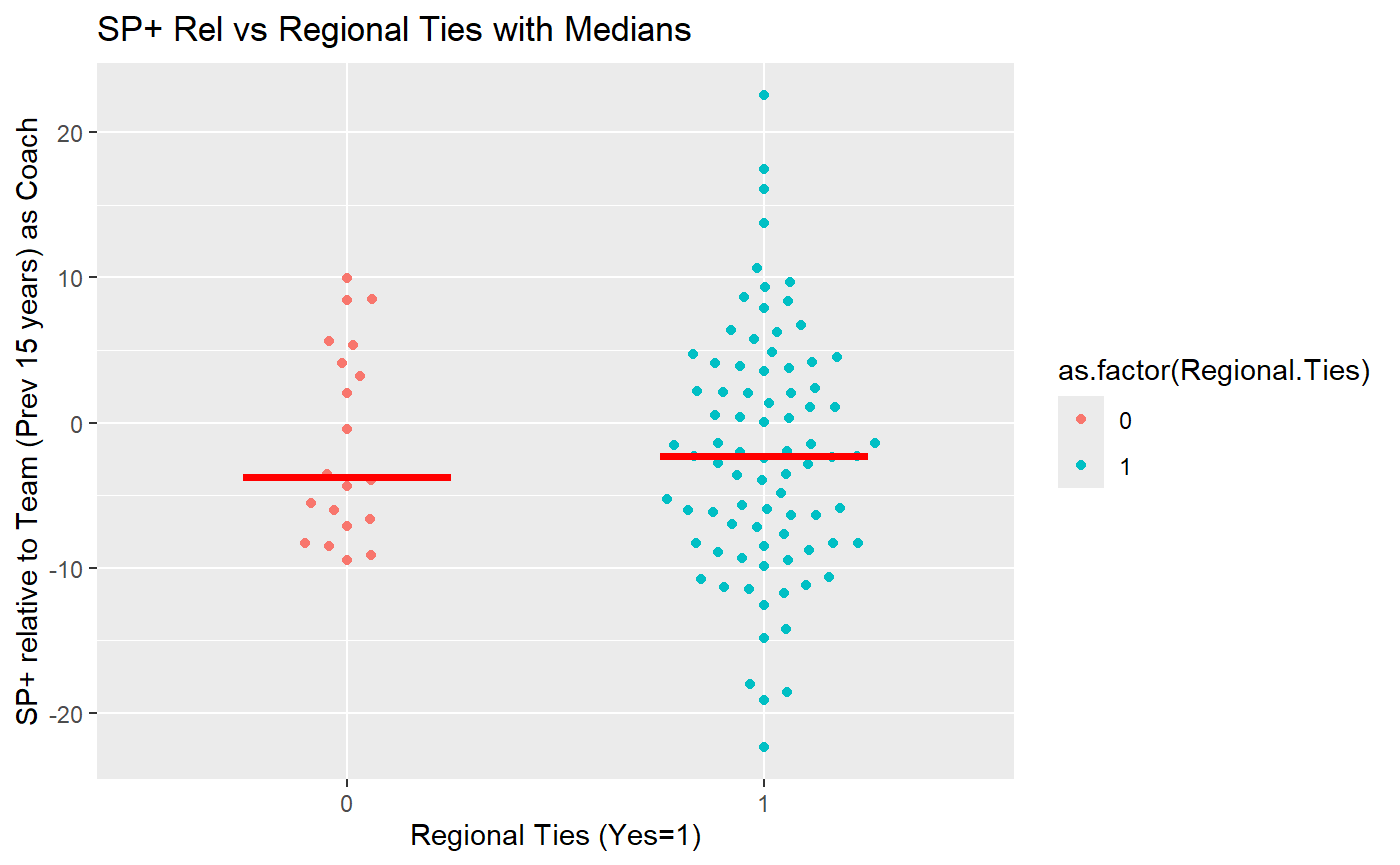
\includegraphics[width=0.4\linewidth,height=\textheight,keepaspectratio,alt={Regional Ties}]{img/cfb_sp_vs_RegionalTies.png}

\end{minipage}%

\caption{\label{fig-cat1}Plots for selected categorical predictors vs SP
Rel +}

\end{figure}%

To determine how successful each coach was as a hire we calculated their
performance as a HC relative to the historical performance of the
university where they were hired. For performance we considered three
measurements. First we considered a hire's win percentage since winning
is arguably the most important outcome for a head coach. Second, we
considered a coach's average Simple Rating System (SRS). This metric,
SRS, is a ``weighted scoring margin'' where the weighted part is based
upon the quality of the teams that have been played \citep{intro_srs}.
Third, we considered a coaches average relative SP+ which is a
predictive metric developed by Bill Connelly \citep{intro_sp} that is a
``tempo- and opponent-adjusted measure'' of team efficiency
\citep{sp_2025}. The historical values for win percentage, SRS and SP+
were obtained using the \emph{cfbfastr} package \citep{cfbfastr}. We
augmented those data with wins and losses from the 2025 season.

{

\begin{longtable}[]{@{}
  >{\raggedleft\arraybackslash}p{(\linewidth - 10\tabcolsep) * \real{0.0714}}
  >{\raggedright\arraybackslash}p{(\linewidth - 10\tabcolsep) * \real{0.2143}}
  >{\raggedright\arraybackslash}p{(\linewidth - 10\tabcolsep) * \real{0.2143}}
  >{\raggedleft\arraybackslash}p{(\linewidth - 10\tabcolsep) * \real{0.1143}}
  >{\raggedleft\arraybackslash}p{(\linewidth - 10\tabcolsep) * \real{0.1429}}
  >{\raggedleft\arraybackslash}p{(\linewidth - 10\tabcolsep) * \real{0.2429}}@{}}

\caption{\label{tbl-top-bottom}Top 10 and Bottom 10 Coaching
Performances Based Upon SP+ Rel}

\tabularnewline

\toprule\noalign{}
\begin{minipage}[b]{\linewidth}\raggedleft
Rank
\end{minipage} & \begin{minipage}[b]{\linewidth}\raggedright
Coach
\end{minipage} & \begin{minipage}[b]{\linewidth}\raggedright
School
\end{minipage} & \begin{minipage}[b]{\linewidth}\raggedleft
SP+ Rel
\end{minipage} & \begin{minipage}[b]{\linewidth}\raggedleft
SP+ Rel Z
\end{minipage} & \begin{minipage}[b]{\linewidth}\raggedleft
Seasons as Coach
\end{minipage} \\
\midrule\noalign{}
\endhead
\bottomrule\noalign{}
\endlastfoot
1 & Curt Cignetti & Indiana & 26.5 & 3.25 & 2 \\
2 & Josh Heupel & UCF & 21.1 & 2.59 & 3 \\
3 & Sonny Dykes & SMU & 17.8 & 2.18 & 5 \\
4 & Rhett Lashlee & SMU & 17.0 & 2.08 & 4 \\
5 & Mike Gundy & Oklahoma State & 13.8 & 1.69 & 21 \\
6 & Mike Elko & Duke & 10.7 & 1.31 & 2 \\
7 & Dabo Swinney & Clemson & 10.2 & 1.26 & 18 \\
8 & Matt Campbell & Iowa State & 10.1 & 1.23 & 10 \\
9 & Bret Bielema & Illinois & 9.3 & 1.14 & 5 \\
10 & Lane Kiffin & Ole Miss & 9.2 & 1.13 & 6 \\
108 & Kalen DeBoer & Alabama & -11.5 & -1.41 & 2 \\
109 & Ryan Walters & Purdue & -11.7 & -1.44 & 2 \\
110 & Brent Pry & Virginia Tech & -13.0 & -1.59 & 4 \\
111 & Deshaun Foster & UCLA & -13.2 & -1.62 & 2 \\
112 & Jonathan Smith & Michigan State & -13.5 & -1.66 & 2 \\
113 & Luke Fickell & Wisconsin & -14.8 & -1.82 & 4 \\
114 & Geoff Collins & Georgia Tech & -16.3 & -1.99 & 4 \\
115 & Chad Morris & Arkansas & -18.0 & -2.20 & 3 \\
116 & Willie Taggart & Florida State & -19.1 & -2.34 & 2 \\
117 & Troy Taylor & Stanford & -21.5 & -2.64 & 2 \\

\end{longtable}

}

\textsubscript{Source:
\href{https://schuckers.github.io/cignetti-noise-paper/index.qmd.html}{Article
Notebook}}

One of the significant challenges for this type of analysis is to define
success. This is certainly the case here, and in no small part is due to
the expectations for each school. What might be a successful record at
Arizona, might not be a success at Alabama. What gets a coach an
extension in College Park, might be a reason to be fired in College
Station or State College. Consequently, our definition of coaching
performance is relative (to team history) rather than absolute.

For relative performance, we took the trimmed mean {[}
`mean(x,trim=0.1)'{]}\{style=``font-family: `Courier New';\u0022\} in R)
of the middle 80\% of years of the performance metric for their time as
a head coach and subtracted the team average of that same metric for the
fifteen years before the coach was hired. We chose to use SP+ as our
measure and we refer to \emph{SP+ Rel} as our outcome variable below.
Note that the correlation between SRS relative to past team performance
and SP+ relative to past team performance was 0.95, results using the
former as a response are likely to be very similar to those for the
latter and so we did not consider models with different responses. The
correlation between \emph{SP+ Rel} and a winning percentage relative to
past teams was 0.82.

Using the R package \emph{cfbfastr}, we obtained historical team data
including wins and losses through the 2024 season as well as SRS and SP+
ratings into the 2025 season. We manually added wins and losses for the
2025 season. All of these data can be found at:
\url{https://github.com/schuckers/cignetti-noise-paper}. Data on
coaching performance is complete through midday on November 13, 2025.

Among these 117 college football head coaching hires in our data, there
were 58 who left a job as head coach (HC) at another school, and 73 of
our hires had been a HC at some level previous to their being hired.
Thirty of the hired coaches had been Defensive Coordinators (DCs) and 17
were Offensive Coordinators (OCs). The other previous positions included
four position coaches, an offensive analyst, four Associate or Assistant
HCs and one hire who was not employed in football. While more coaches
were hired directly from DC positions, 45 of the 117 hires (38\%) had
defense as their background. Seventy-three (73 of the hires had been a
head coach at the college or NFL previously, while 26 had previously
coached in the NFL. Thirty percent of the coaches were hired to jobs
within the same conference. Only 18 of our hires were promoted from the
coaching staff of the same institution. The average age of our coaches
when they were hired is approximately 47 years.

The majority of hired coaches, 74, had not worked for, played at or
attended the school that hired them. While the vast majority of the
hired coaches played college football, just under 50\% of them, 56,
played for a P4 school and only 12 played in the NFL.

Below when we refer to recent metrics we will be talking about a five
year period and when we refer to previous metrics we will be talking
about a 15 year period.

\begin{figure}

\begin{minipage}[t]{0.50\linewidth}

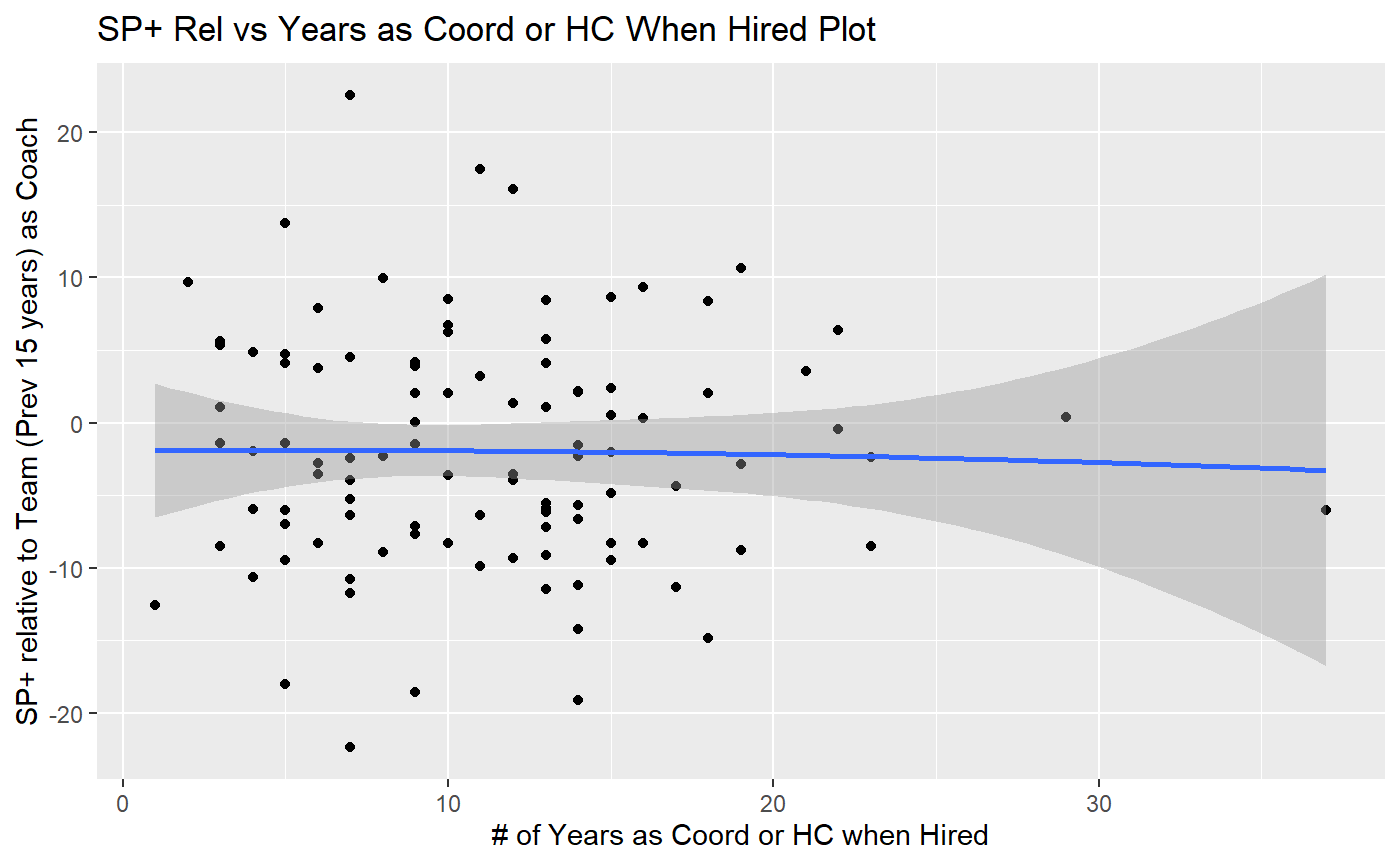
\includegraphics[width=0.3\linewidth,height=\textheight,keepaspectratio,alt={Numb. years as Coord or HC}]{img/cfb_sp_vs_numb_yrs_Coord_HC_quad.png}

\end{minipage}%

\caption{\label{fig-numeric1}Plots for selected numeric predictors vs SP
Rel}

\end{figure}%

Next we will look at some of relationship between our variables and our
measure of coaching performance, \emph{SP+ Rel}. Table~\ref{tbl-var}
contains the list of predictor variables as well as their definitions.
Turning to the graphics, we see a sampling of these relationship in
Figure~\ref{fig-cat1}. In that figure, we can see that medians (red
lines) seem to indicate there are some differences between the
categories for winning a national championship as a coordinator,
\textbf{?@fig-prev-nc}, and for previous job was as an OC,
\textbf{?@fig-oc}. Otherwise the other variables do not seem to suggest
there is much difference in the typical coaching performance for the
different characteristics recorded in those subfigures. More graphics
like these can be found for the other categorical predictors in
Figure~\ref{fig-append-cat} and Figure~\ref{fig-append-cat2}. In those
graphics, Figure~\ref{fig-append-cat} (d) suggests that having played in
the NFL yields a higher median \emph{SP+ Rel} as does having previously
won a national championship as a coordinator,
Figure~\ref{fig-append-cat2} (b). However, quite a bit fewer coaches
have the value that is associated with the higher median.

Turning to numeric predictors, we can see the relationship between
\emph{SP+ Rel} and four of these predictors in
Figure~\ref{fig-numeric1}. In \textbf{?@fig-yrs-coord}, we can see that
there is not a relationship between number of years as a HC or
Coordinator before being hired. The three remaining subfigures,
\textbf{?@fig-age}, \textbf{?@fig-sp-recent}, \textbf{?@fig-sp-prev15},
also show negative linear relationships between \emph{SP+ Rel} and
coach's age, teams performance in the recent past, 5 years, and team
performance in the previous 15 years. More figures like this can be
found in Figure~\ref{fig-append-numeric} of the Appendix at the end of
this report. Noteworthy among those figures in the Appendix is that
there seems to be a positive linear relationship between a hired coach's
\emph{SP+ Rel} and their previous \emph{SP+ Rel} had they been a college
HC previously.

Model and Results

The goal of this analysis is to build a predictive model for the success
of a coaching hire and to identify the factors that impact that success.
We selected 29 predictors found in Table~\ref{tbl-var} that could be
useful for predicting coaching success. For our model formulation, we
chose to build a regularized linear regression model for SP+ relative to
past team performance, hereafter \emph{SP+ Rel}. We used
\texttt{cv.glmnet} as part of the \texttt{glmnet} library in R
\citep{glmnet}. For our regularization, we considered both ridge and
lasso regression, and we used 8-fold cross validated performance to
determine the regularization/shrinkage parameter, \(\lambda\), for our
model. We ran 20 different randomizations of 8-fold cross validation.
Consistently, across all these different randomizations of the folds, we
found that the best lasso model had a smaller out of sample prediction
error (via MSE) than the best ridge model. To get the parameter
coefficient estimates discussed below we fit the full model via a lasso
with \(\lambda\) set to the average of the shrinkage parameters that
minimized the cross-validation error. In fact there was no variability
in these shrinkage parameters across the 20 randomizations. Because some
of our predictors, e.g.~\texttt{sp\_prev\_rel}, were available only if a
coach had previously been a college HC, we included whether or not a
coach was previously an HC in all of the models we considered.

Our final prediction equation is:

\[\hspace{-4in} SP+ Rel = 0.88 -0.42 \text{ Was College HC before at any level} + \]
\[2.37 \text{ Previous job was as an OC} - 0.34 \text{ Hiring School's Team SP+ Rel in 15 years before hiring}\]
\{\#eq-predictioneq\}

The largest factors in our model were whether or not the coach's
previous job was as an OC (\texttt{PreviousOC}), whether they had ever
been a college coach previously (\texttt{prevCollegeHC}) and the team's
performance over the last 15 years (\texttt{team\_sp\_prev}). Having
been hired from an OC position is associated with about a \(2.37\) point
increase in a coach's \emph{SP+ Rel}. While if a hire was previously a
college football HC, the predicted decrease in their team's performance
is fourth-tenths a point. The last term in our prediction equation
involves a team's average \emph{SP+ Rel} over the previous 15 years and
that is negatively associated with how a coaching hire's teams will
perform. We can interpret the value here of \(-0.34\) as the expected
decrease in a team's average performance for every additional point of
\emph{SP+ Rel} that the hiring team had over the previous 15 years. This
is a regressive effect, since SP+ for an average team should be around
zero, then for a new coaching hire, good teams we would expect them to
get worse and very good teams we would expect them to get much worse,
while for below average teams we would expect them to get better just by
making the hire. One possible explanation for this is a regression to
the mean as team performance tends to move to the average of all teams,
which for SP+ is around zero. Another explanation is college football
has moved to an era of more parity and relative coaching performance is
not immune to moving with that trend.

The hires with the ten highest and ten lowest predicted \emph{SP+ Rel}
are listed in Table~\ref{tbl-top-bottom}. We can see that the model
suggests that the hire with the highest predicted success was Rhett
Lashlee at SMU. Eight of the ten top predicted \emph{SP+ Rel} values had
positive observed values. Tony Elliott at Virginia and Jedd Fisch at
Arizona were the exceptions. Elliott has improved his Virginia teams
and, if he stays, may yet get to positive territory. Fisch left Arizona
after a successful second season. Among the coaches predicted to have
negative \emph{SP+ Rel}, eight of the ten are in or have finished in
negative territory. The exceptions are Dan Mullen whose team performance
dropped significantly over his four years at Florida and Kirby Smart who
has impressively elevated Georgia to new heights. Seven of these ten
coaches have already been fired with only Smart, Fickell and Venables
still employed at these schools. Venables' Oklahoma 2025 team had one of
their best recent seasons with him as a HC and so there is hope for a
turnaround there. Looking at the bottom ten schools, most of the schools
there are considered to be `elite' or nearly so. The model predicts that
succeeding at these schools is hard partly because they are already at
the upper tail of the distribution. Overall the model accurately
predicts whether a coach will have a positive or negative \emph{SP+ Rel}
67\% of the time.

The model we have explains about \(15\%\) of the variability in the
team's performance with a newly hired coach and the average difference
between our model's prediction and the actual \emph{SP+ Rel} of the
coaches in these data is just over \(7.5\) points. That is a large
amount of variability and it speaks to the noisiness of these data.
However, the model does well given that noisiness at predicting who will
have a \emph{SP+ Rel} above or below zero achieving 68\% accuracy on
this metric.

While it is important to focus on the factors that do influence hiring
success, it is worth mentioning those that do \textbf{not} given the
factors that \textbf{are} in the model. Having a previous connection to
the school, being a previous head coach at any level, having NFL
coaching experience, having experience as a recruiting coordinator,
having played football in the NFL or at a P4 school seem to have no
impact on our ability to predict how well a coach will do. Winning a
national championship as a HC at any level as well as being a
Coordinator for a team that won a national championship or a conference
championship does not predict coaching success. Similarly having
regional ties to the hiring school does not seem to be impactful and the
same is true for moving within the same conference or leaving a P4
school. A coach's relative SP+ as a previous HC is also not predictive,
as is their previous win percentage. One possible explanation is that we
are taking averages of previous coaching performance that misses changes
in SP+ over a coach's time with a previous school, e.g.~Matt Rhule at
Temple and Lance Leipold at Buffalo. Finally, the number of games
coached as an HC before being hired is unimportant as a predictor as is
the recent winning percentage of the team.

Discussion

Choosing a successful P4 college football coach is a difficult task. In
this paper we have collected data on recent P4 coaching hires and built
a predictive model for their performance. The data we used was on recent
P4 hires and we measured their performance using average SP+ relative to
previous performance of the school's teams, \emph{SP+ Rel}. As mentioned
above \emph{SP+ Rel} is correlated with a coach's winning percentage and
highly correlated with their SRS, the other statistical measure of team
performance that we considered.

Ultimately, we found that there are several factors that are predictive
of the performance of a college football head coaching hire. These
factors include whether a hire had been a previous college coach,
whether the hire had previously won a conference championship as a
coach, whether their prior job was as an offensive coordinator, their
age and the quality of the team they were hired to lead over the
previous 15 years. Our prediction model does not perform particularly
well, only explaining just under a quarter of the variability in
coaching performance.

The 2020 season is among the years in these data. The effects of COVID
were felt across college football in the form of shortened seasons and
empty stadiums. Every school and every conference handled the situation
differently. One of the choices we made as part of this analysis was
that we would keep the 2020 season in our data. Given the short tenure
of some college football head coaching hires, we felt having as much
data as possible was important.

This study measured the success of a coaching hire by how they did on
average relative to their team's previous 15 years. That is not a
perfect measure. Team performance fluctuates and trends, sometimes
upward and sometimes downward. Ideally when a new coach is hired their
teams trend upward as they recruit players that fit their system and
they become comfortable in their new job. An average over a short period
may miss this effect. That said, it is very difficult to generate a
measure of coaching success that captures all of the possible nuances.
Therefore, we chose to stick with an average relative to past team
performance.

Much has been made about the recent success of Curt Cignetti and he has
done an amazing job as the HC at Indiana. Cignetti is an outlier. It is
very clear which observations corresponds to the exceptional job
Cignetti has done at Indiana. That said, an outlier is not a trend and
the signal from these data is weak. Hiring a coach is hard; hiring a
really successful coach is \emph{very} hard. There are no magic
attributes, at least \emph{not} among the factors we investigated, that
guarantee future success. The data as can be seen in
Figure~\ref{fig-cat1} through Figure~\ref{fig-append-numeric} is very
noisy and the trends, while tempting, are mild. Great coaches are hard
to find and many schools find themselves having difficulty
distinguishing the Cignetti's from the noise.

The code and the data for the analyses presented here can be found at
\url{https://github.com/schuckers/cfb_coach_analytics}.

Thanks to the team of folks who put together \texttt{cfbfastr} for
making their data available in a usable and regularly updated manner and
to Brian Macdonald (Yale) for thoughtful discussions about this
analysis.

Appendix

\begin{longtable}[]{@{}
  >{\raggedright\arraybackslash}p{(\linewidth - 2\tabcolsep) * \real{0.5000}}
  >{\raggedright\arraybackslash}p{(\linewidth - 2\tabcolsep) * \real{0.5000}}@{}}
\caption{List of variables used as predictors in this paper. All values
are relative to the coach at the time they were
hired.}\label{tbl-var}\tabularnewline
\toprule\noalign{}
\begin{minipage}[b]{\linewidth}\raggedright
Variable Name
\end{minipage} & \begin{minipage}[b]{\linewidth}\raggedright
Variable Meaning
\end{minipage} \\
\midrule\noalign{}
\endfirsthead
\toprule\noalign{}
\begin{minipage}[b]{\linewidth}\raggedright
Variable Name
\end{minipage} & \begin{minipage}[b]{\linewidth}\raggedright
Variable Meaning
\end{minipage} \\
\midrule\noalign{}
\endhead
\bottomrule\noalign{}
\endlastfoot
\texttt{prevCollegeHC} & Were they previously a college head coach
(HC) \\
\texttt{PreviousHC} & Was job when hired as a HC \\
\texttt{PreviousOC} & Was job when hired as an Offensive Coordinator
(OC) \\
\texttt{PreviousDC} & Was job when hired as a Defensive Coordinator
(DC) \\
\texttt{Conf.LeavingP4} & Was job when hired at P4 school \\
\texttt{SameConf} & Was job when hired in same conference \\
\texttt{AgeAtHiringMinus50} & Age on Jan 1 of first season as HC \\
\texttt{ConnectionToHiring.School} & Had coach previously played or been
employed at hiring school \\
\texttt{NFLCoachingExperience} & Had the coach ever coached in the
NFL \\
\texttt{RecruitingCoord} & Previously been a recruiting coordinator or
not \\
\texttt{PlayedNFL} & Had coach played in the NFL \\
\texttt{Played.Power.4} & Had coach played at a Power 4 school \\
\texttt{WonNCasHCany} & Had coach won a National Championship (NC) as HC
at any level (college) \\
\texttt{WonCCasHCany} & Had coach won a Conference Championship (CC) as
HC at any level (college) \\
\texttt{WonNCasCoordAny} & Had coach won a NC as an OC, DC, or AHC at
any level (college) \\
\texttt{WonCCasCoordAny} & Had coach won a CC as an OC, DC, or AHC at
any level (college) \\
\texttt{SideO} & Is coach's primary background on Offense \\
\texttt{LeavingNFL} & Was previous job in the NFL \\
\texttt{Regional.Ties} & Had coach previously worked within 500 miles of
hiring school \\
\texttt{numb\_years\_Coord\_adj} & Number of years as OC/DC/AHC/HC above
average of 11.8 years \\
\texttt{numb\_years\_Coord\_HCadj2} & Numbers of years as OC/DC/AHC/HC
different from 11.8 squared \\
\texttt{PromoteWithin} & Coach was promoted to HC from other position at
same school \\
`NumberPriorStops' & Number of different teams coach worked for before
being hired \\
\texttt{AllPriorWinPct} & Win Percent as Coach at all levels before
being hired \\
\texttt{winpct\_prev\_Rel} & Win percent as HC at previous job \\
\texttt{team\_sp\_prev} & Hiring school's SP+ in 15 years before hire \\
\texttt{team\_sp\_recent} & Hiring school's SP+ in 5 years before
hire \\
\texttt{GamesAsHCPrior} & Number of games as a HC before being hired \\
\texttt{team\_winpct\_recent} & Hiring School's win percentage in the
last 5 years \\
\texttt{sp\_prev\_rel} & Previous \emph{SP+ Rel} in HC role \\
\end{longtable}

\begin{figure}

\begin{minipage}[t]{0.50\linewidth}

\centering{

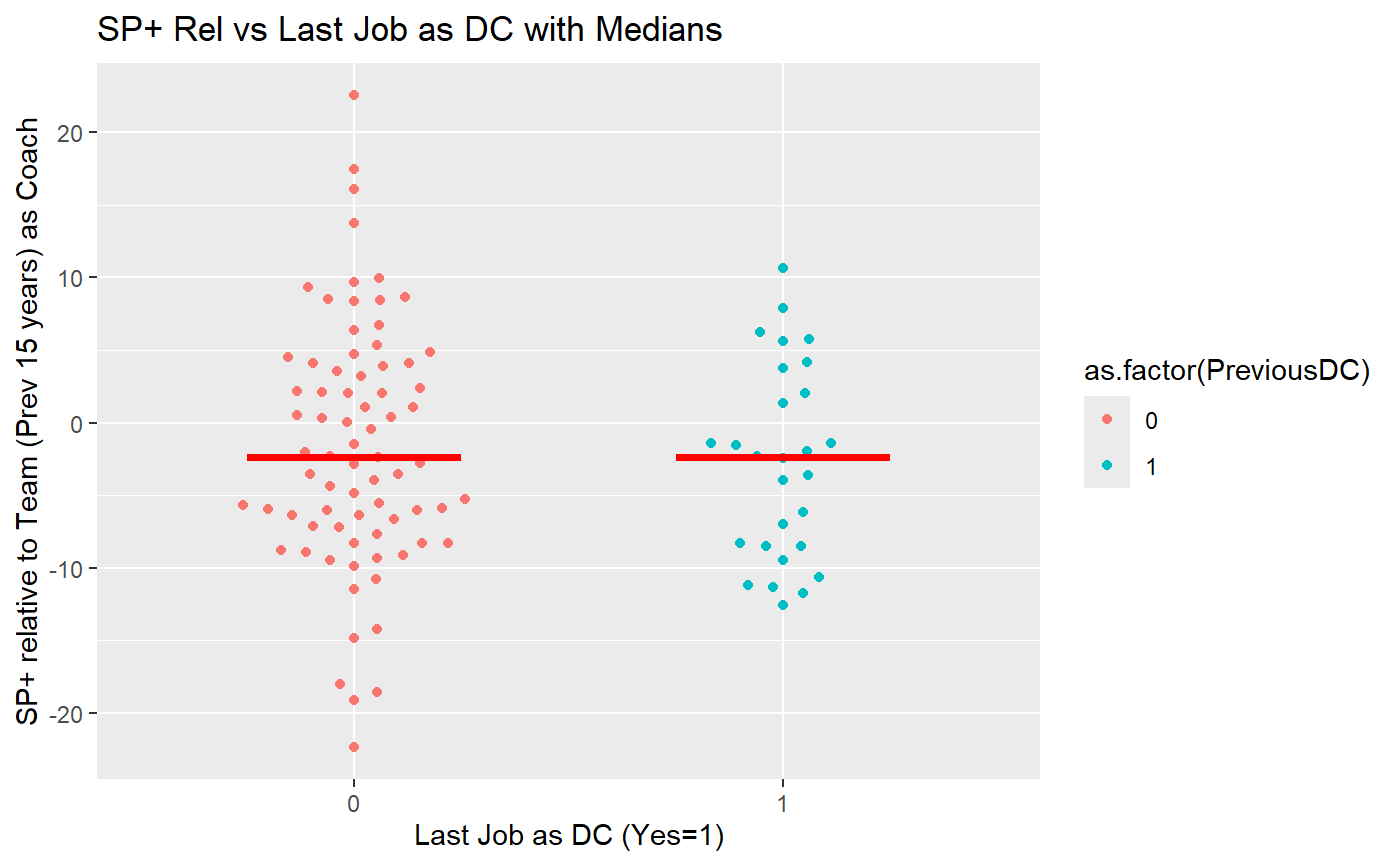
\includegraphics[width=0.4\linewidth,height=\textheight,keepaspectratio]{img/cfb_sp_vs_LastDC.png}

}

\subcaption{\label{fig-last-dc}Previous job as DC}

\end{minipage}%
%
\begin{minipage}[t]{0.50\linewidth}

\centering{

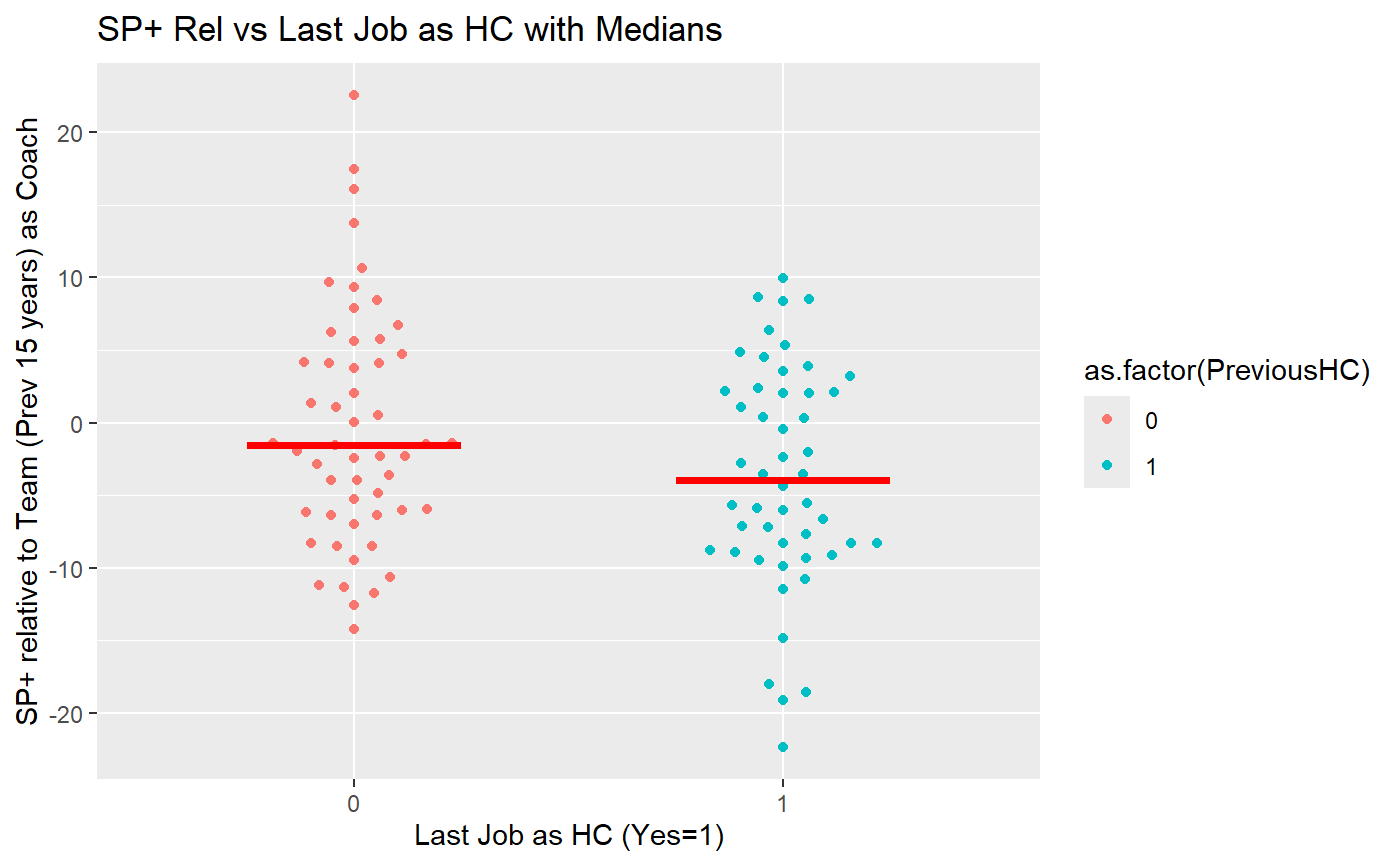
\includegraphics[width=0.4\linewidth,height=\textheight,keepaspectratio]{img/cfb_sp_vs_PreviousHC.png}

}

\subcaption{\label{fig-prev-hc}Previous job as HC}

\end{minipage}%
\newline
\begin{minipage}[t]{0.50\linewidth}

\centering{

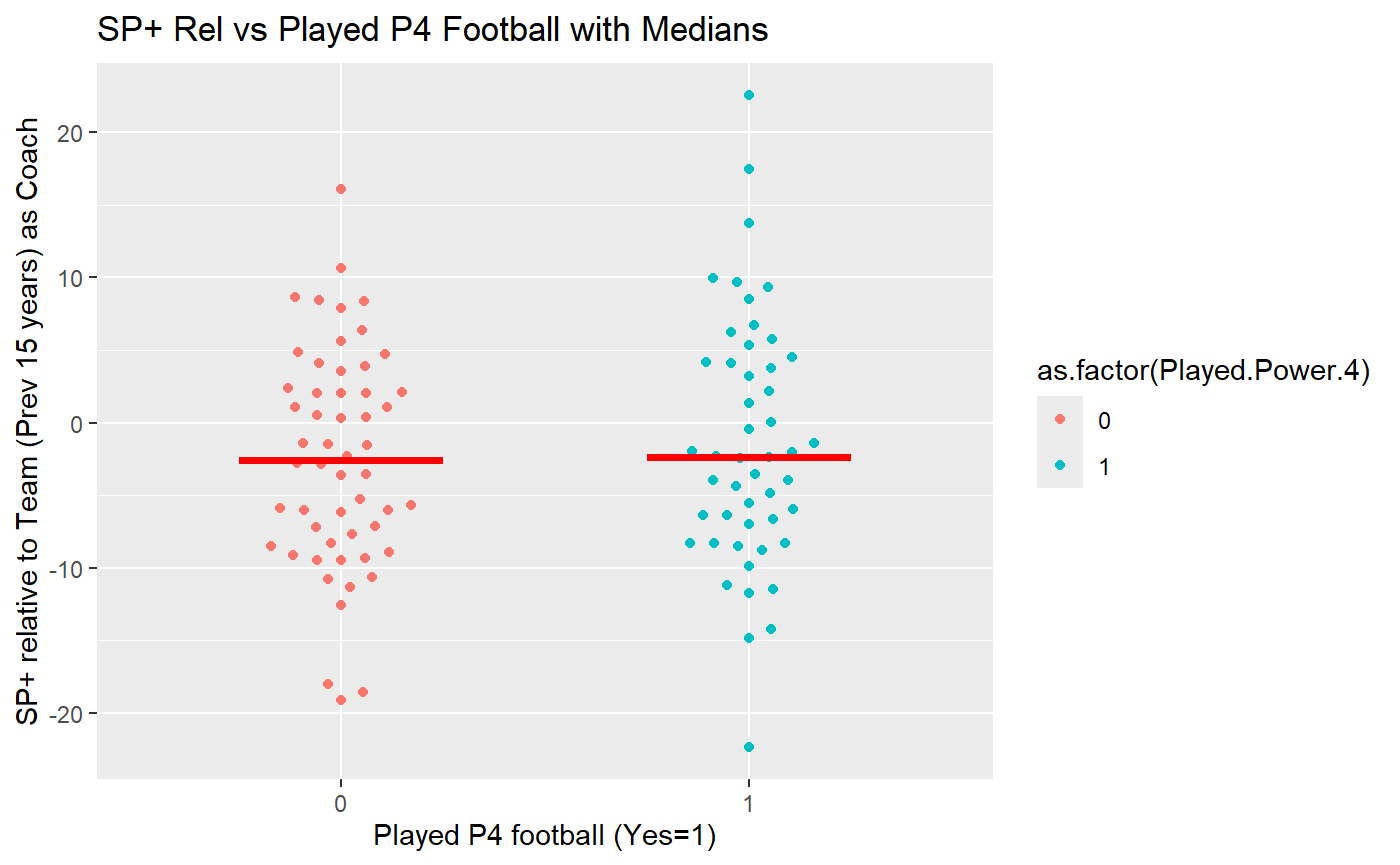
\includegraphics[width=0.4\linewidth,height=\textheight,keepaspectratio]{img/cfb_sp_vs_PlayedP4.png}

}

\subcaption{\label{fig-played-p4}Played P4 football}

\end{minipage}%
%
\begin{minipage}[t]{0.50\linewidth}

\centering{

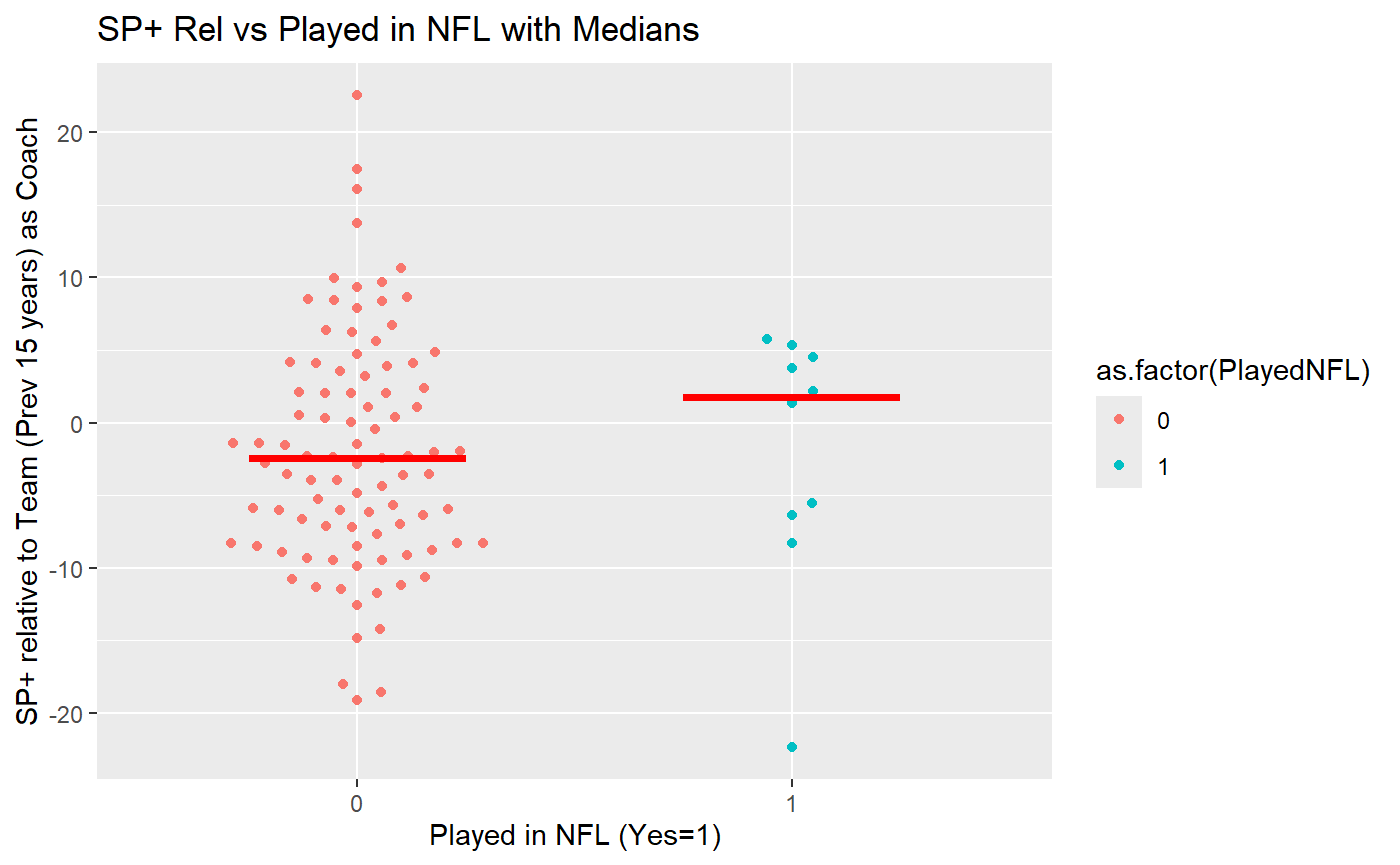
\includegraphics[width=0.4\linewidth,height=\textheight,keepaspectratio]{img/cfb_sp_vs_PlayedNFL.png}

}

\subcaption{\label{fig-played-nfl}Played in the NFL}

\end{minipage}%
\newline
\begin{minipage}[t]{0.50\linewidth}

\centering{

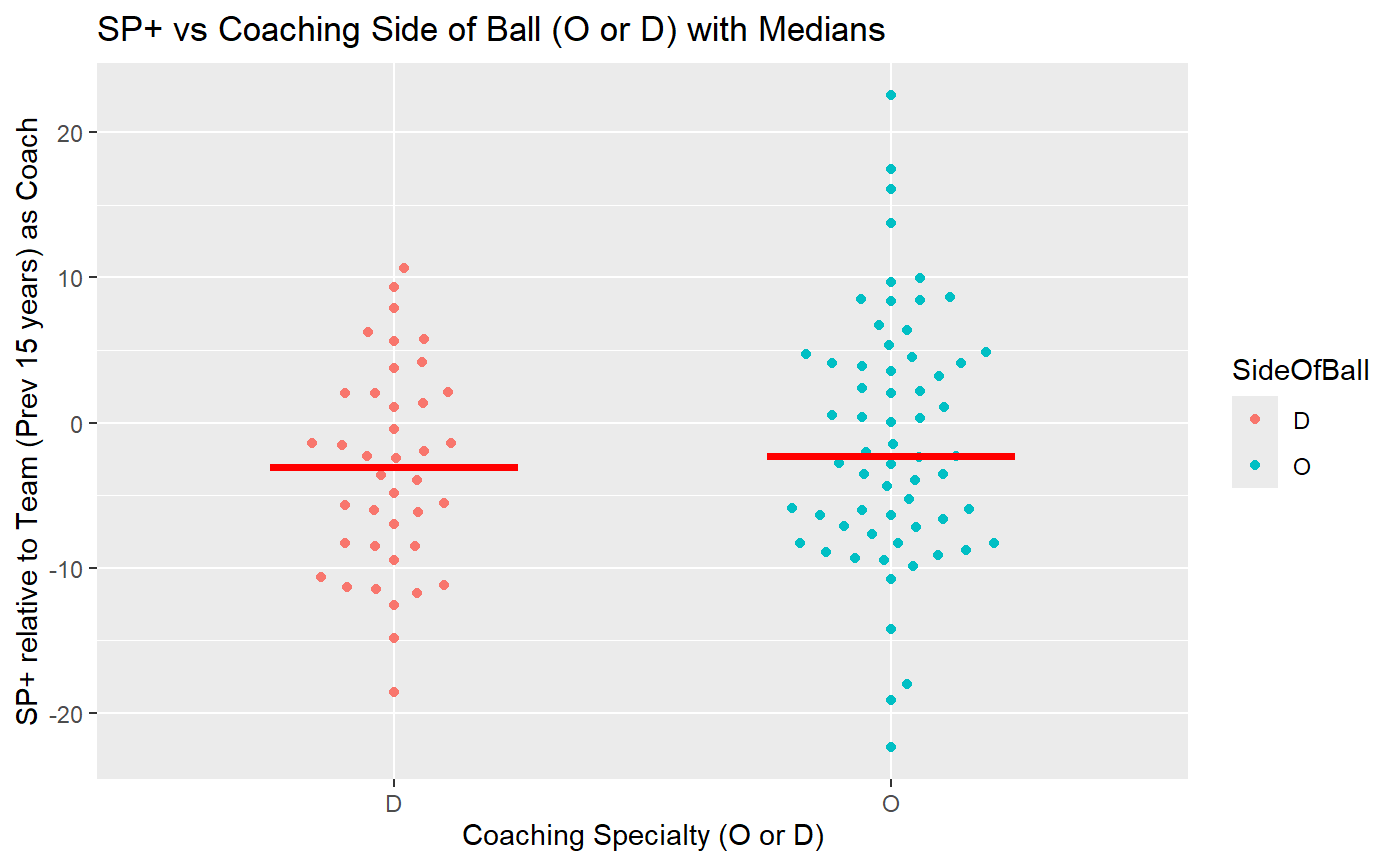
\includegraphics[width=0.4\linewidth,height=\textheight,keepaspectratio]{img/cfb_sp_vs_SideOfBall.png}

}

\subcaption{\label{fig-side-ball}Side of the Ball}

\end{minipage}%
%
\begin{minipage}[t]{0.50\linewidth}

\centering{

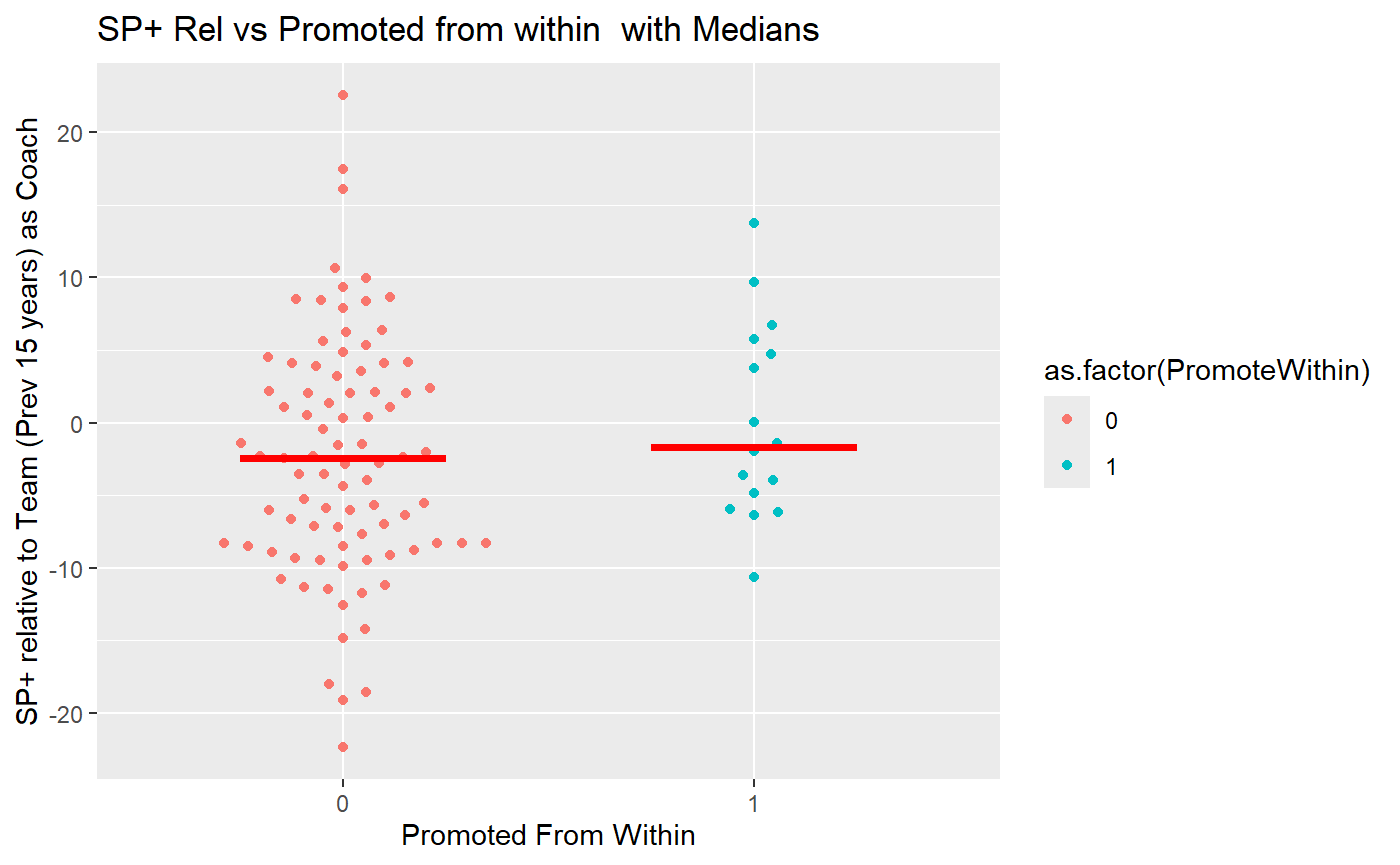
\includegraphics[width=0.4\linewidth,height=\textheight,keepaspectratio]{img/cfb_sp_vs_PromoteWithin.png}

}

\subcaption{\label{fig-promote-within}Promoted from Within}

\end{minipage}%

\caption{\label{fig-append-cat}Additional plots of categorical
predictors vs \emph{SP+ Rel}}

\end{figure}%

\begin{figure}

\begin{minipage}[t]{0.50\linewidth}

\centering{

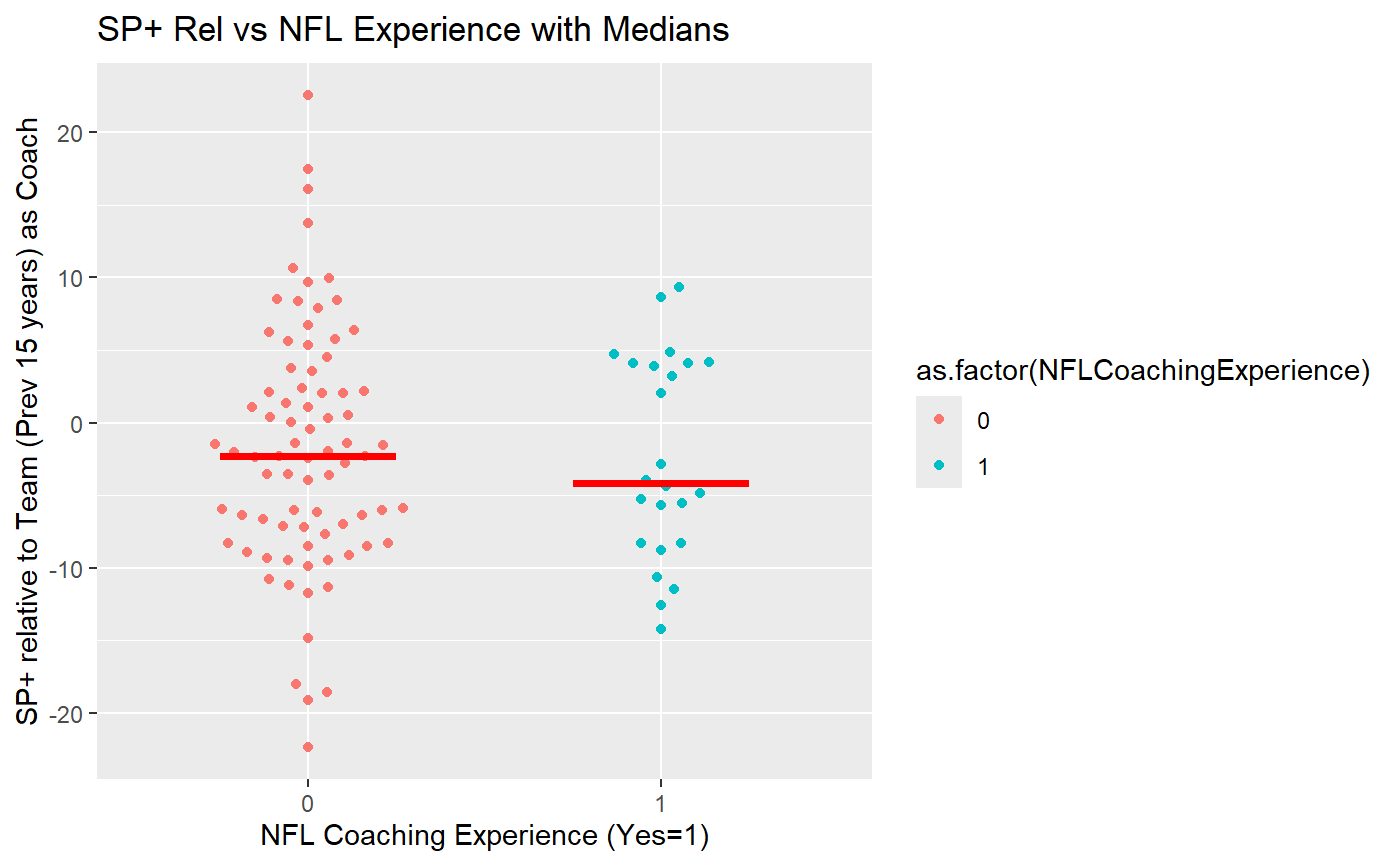
\includegraphics[width=0.4\linewidth,height=\textheight,keepaspectratio]{img/cfb_sp_vs_PrevNFLCoaching.png}

}

\subcaption{\label{fig-nfl-exp}Has NFL coaching experience}

\end{minipage}%
%
\begin{minipage}[t]{0.50\linewidth}

\centering{

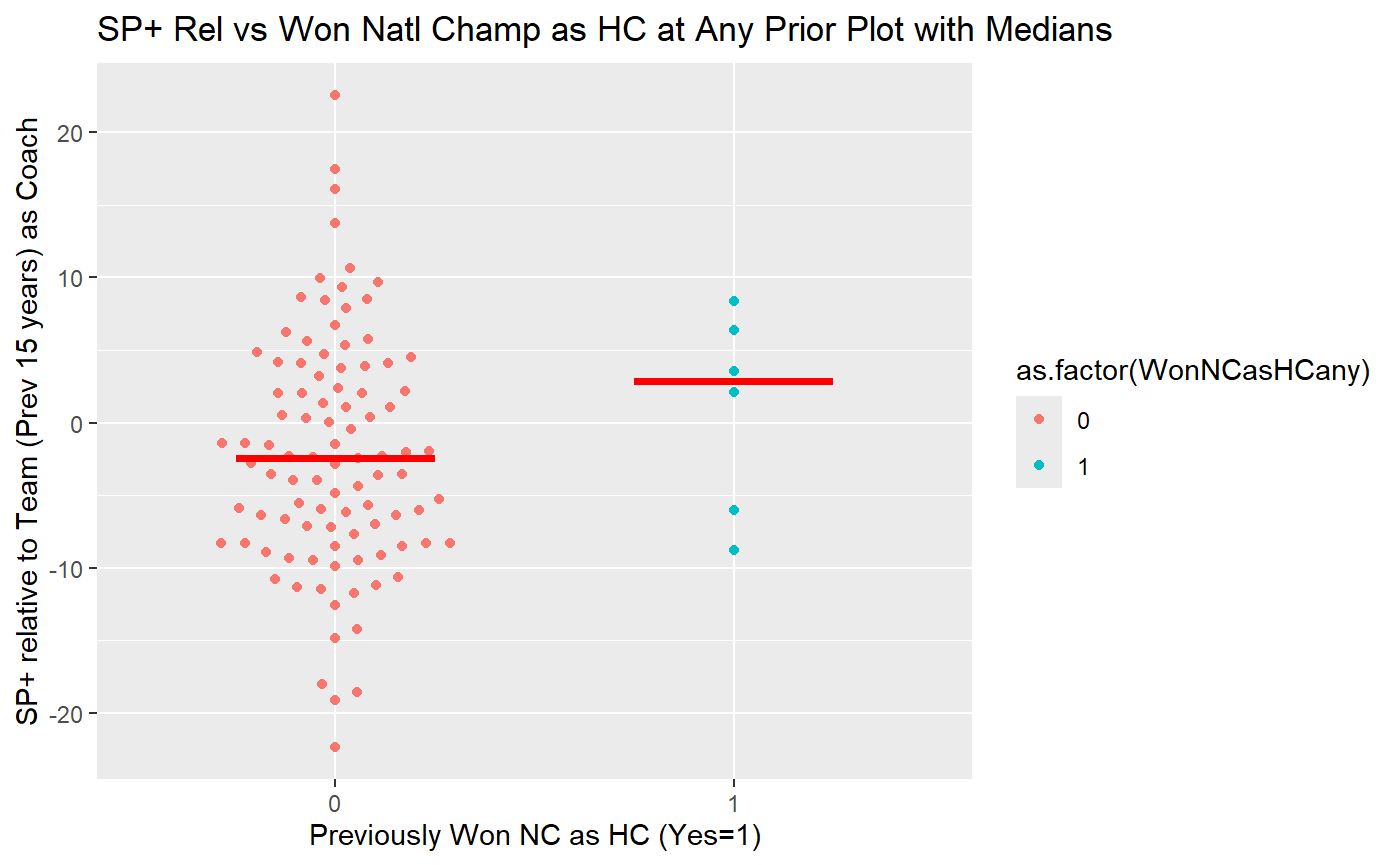
\includegraphics[width=0.4\linewidth,height=\textheight,keepaspectratio]{img/cfb_sp_vs_WonNCasHCAny.png}

}

\subcaption{\label{fig-nc-hc}Won Natl. Champ. as HC any level}

\end{minipage}%
\newline
\begin{minipage}[t]{0.50\linewidth}

\centering{

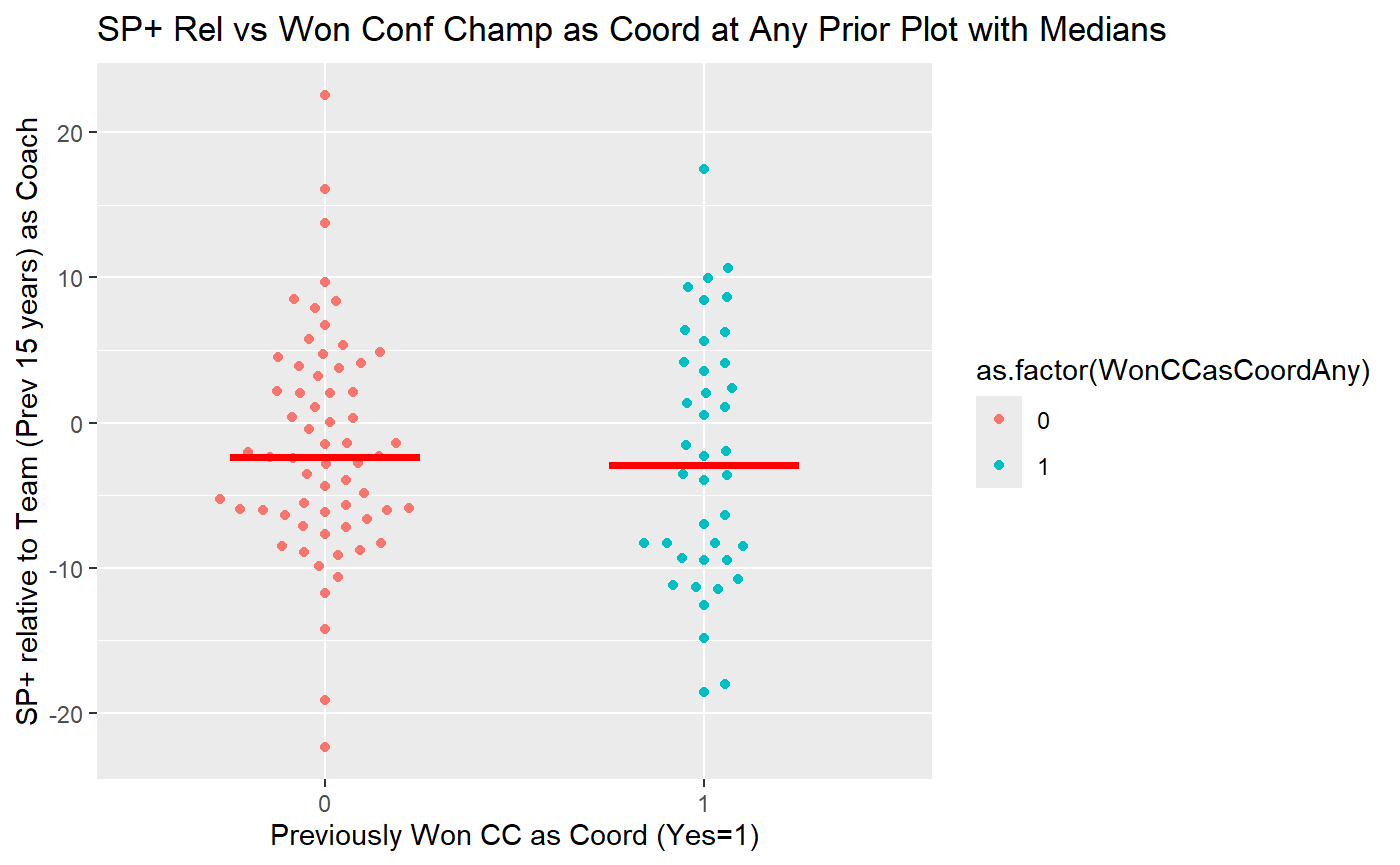
\includegraphics[width=0.4\linewidth,height=\textheight,keepaspectratio]{img/cfb_sp_vs_WonCCasCoordAny.png}

}

\subcaption{\label{fig-cc-coord}Won Conf. Champ. as Coord any level}

\end{minipage}%
%
\begin{minipage}[t]{0.50\linewidth}

\centering{

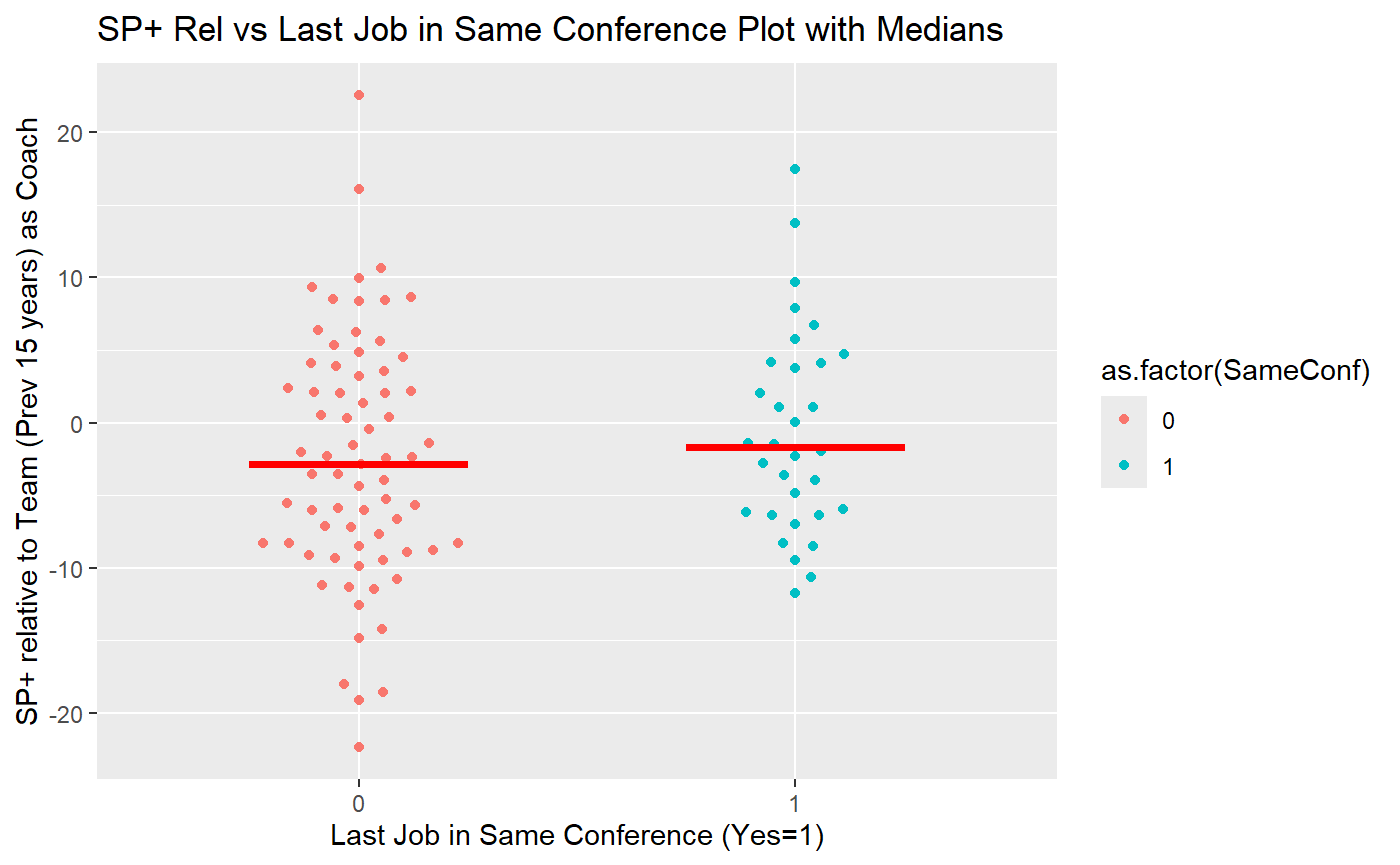
\includegraphics[width=0.4\linewidth,height=\textheight,keepaspectratio]{img/cfb_sp_vs_SameConf.png}

}

\subcaption{\label{fig-same-conf}Hired within same conference}

\end{minipage}%
\newline
\begin{minipage}[t]{0.50\linewidth}

\centering{

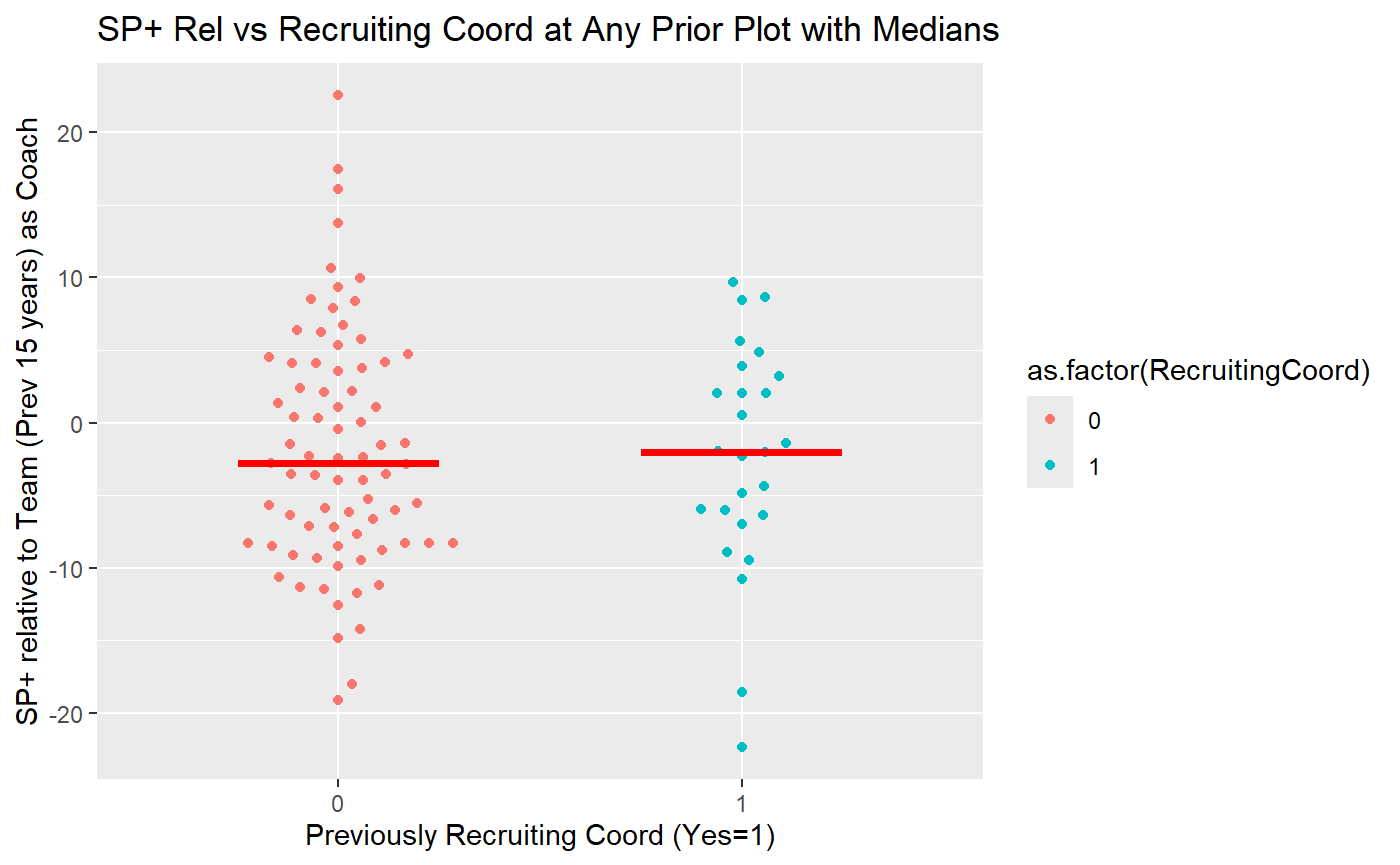
\includegraphics[width=0.4\linewidth,height=\textheight,keepaspectratio]{img/cfb_sp_vs_PrevRecruitCoord.png}

}

\subcaption{\label{fig-recruit-coord}Been Recruiting Coordinator
previously}

\end{minipage}%

\end{figure}%

Additional plots of categorical predictors vs \emph{SP+ Rel}

\begin{figure}

\begin{minipage}[t]{0.50\linewidth}

\centering{

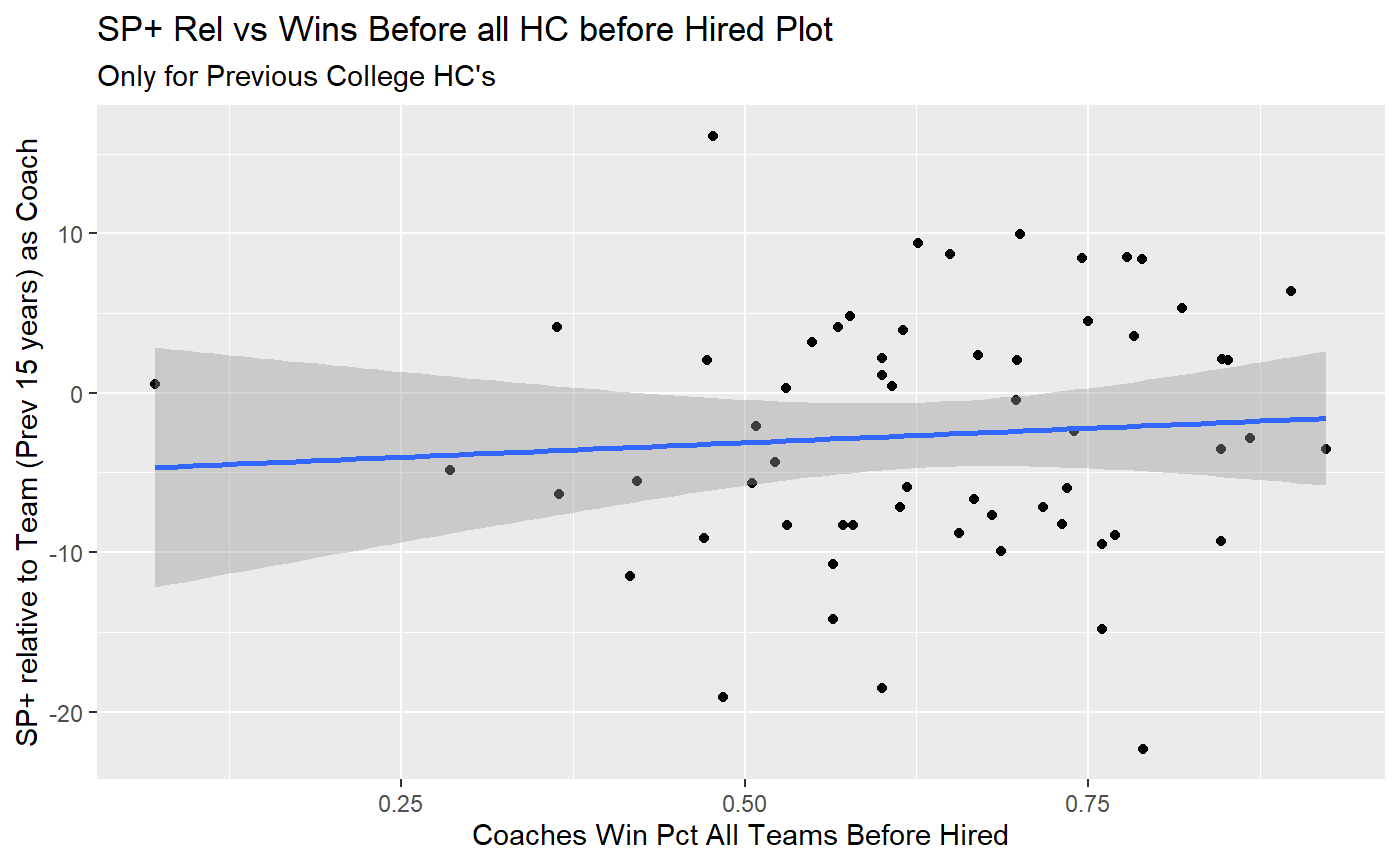
\includegraphics[width=0.4\linewidth,height=\textheight,keepaspectratio]{img/cfb_sp_vs_AllPastWinPctAsHC.png}

}

\subcaption{\label{fig-all-winpct}All Past Win Pct as HC}

\end{minipage}%
%
\begin{minipage}[t]{0.50\linewidth}

\centering{

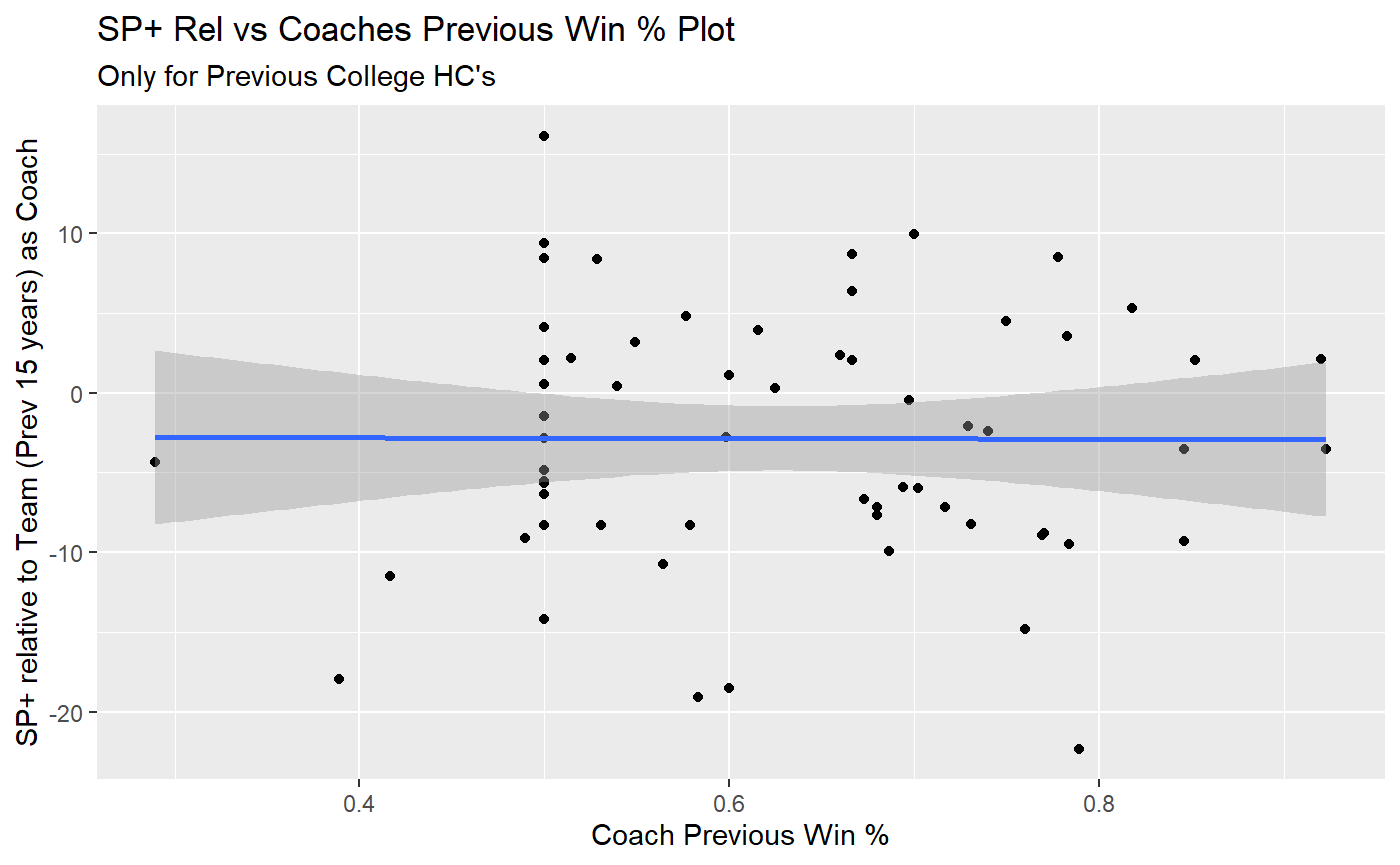
\includegraphics[width=0.4\linewidth,height=\textheight,keepaspectratio]{img/cfb_sp_vs_Coach_PrevWinPct.png}

}

\subcaption{\label{fig-prev-winpct}Win Pct at Previous job if HC}

\end{minipage}%
\newline
\begin{minipage}[t]{0.50\linewidth}

\centering{

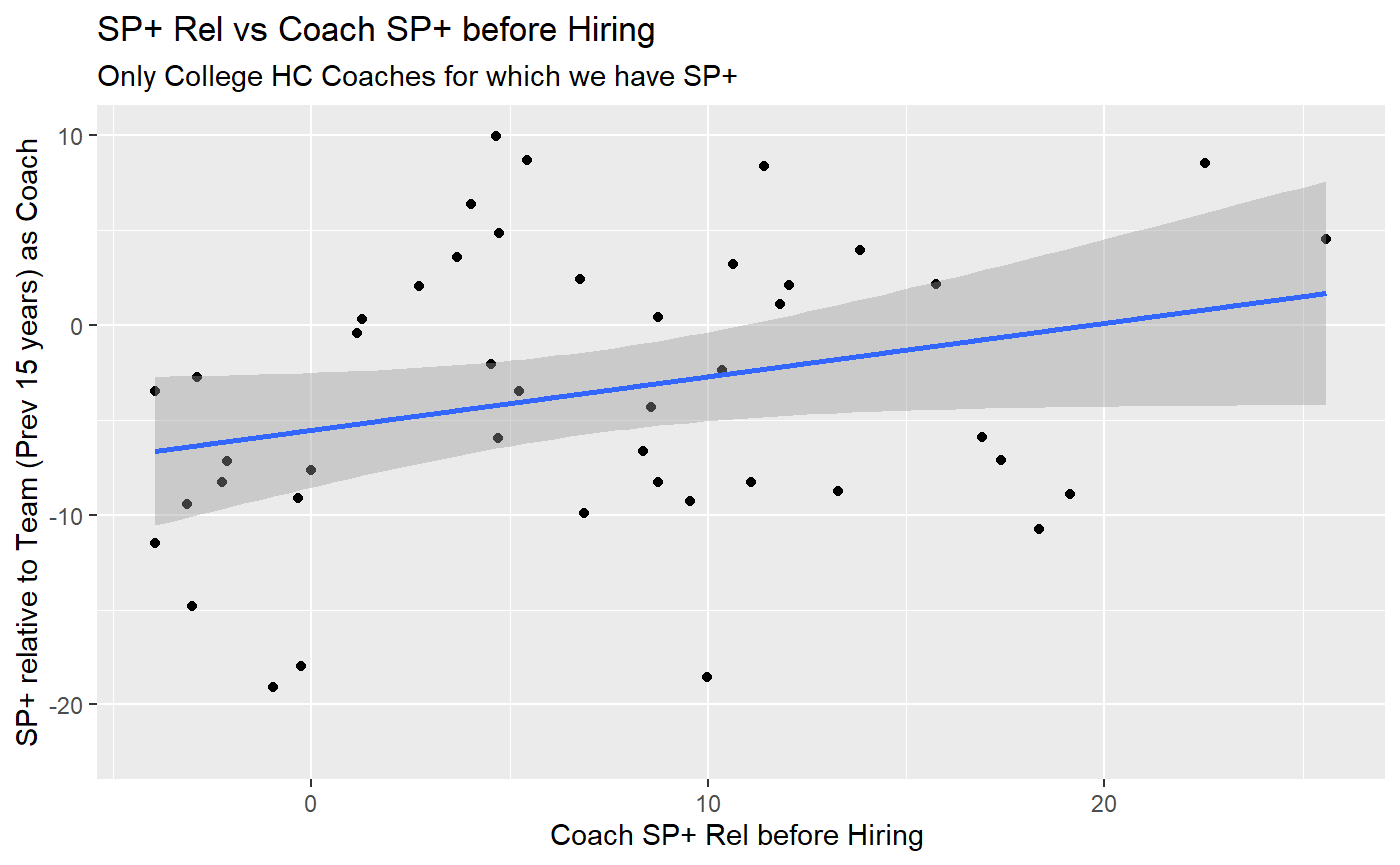
\includegraphics[width=0.4\linewidth,height=\textheight,keepaspectratio]{img/cfb_sp_vs_Coach_sp_rel_before.png}

}

\subcaption{\label{fig-coach-sp-before}Coach \emph{SP+ Rel} before hire}

\end{minipage}%
%
\begin{minipage}[t]{0.50\linewidth}

\centering{

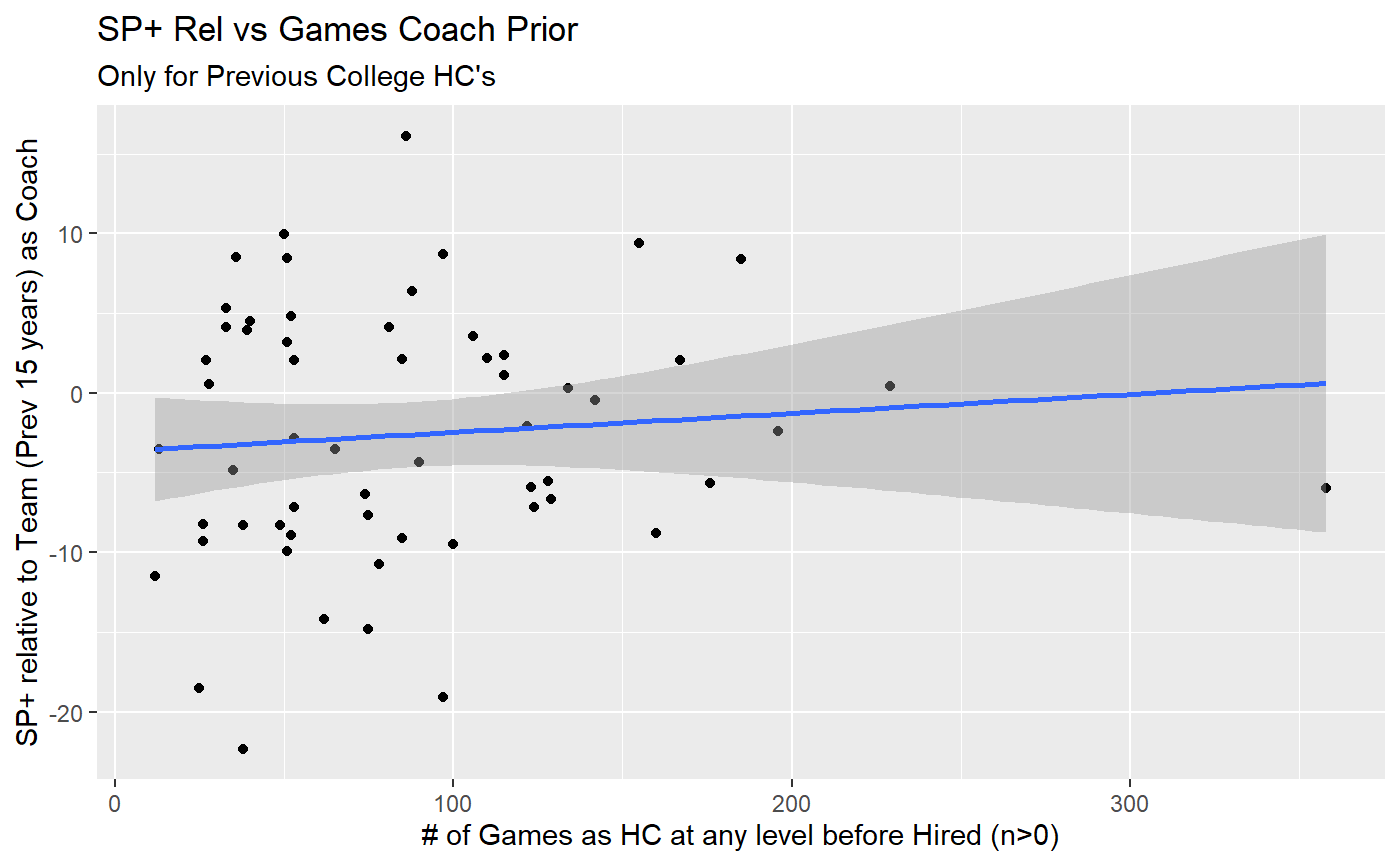
\includegraphics[width=0.4\linewidth,height=\textheight,keepaspectratio]{img/cfb_sp_vs_numb_gamesAsHC.png}

}

\subcaption{\label{fig-games-hc}Numb. of games as HC}

\end{minipage}%
\newline
\begin{minipage}[t]{0.50\linewidth}

\centering{

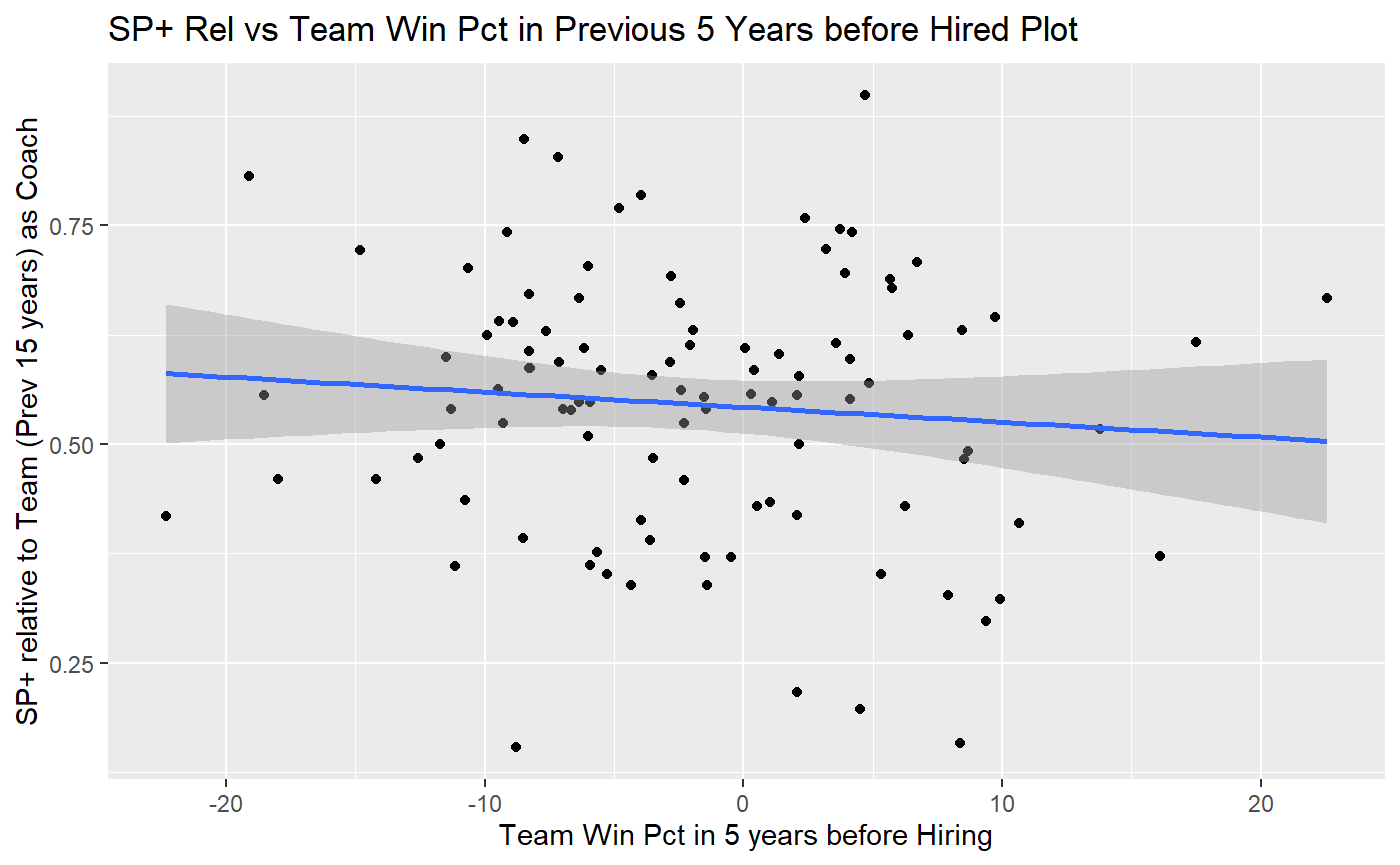
\includegraphics[width=0.4\linewidth,height=\textheight,keepaspectratio]{img/cfb_sp_vs_TeamWinPctRecent.png}

}

\subcaption{\label{fig-team-winpct-recent}Team Win Pct in last 5 years}

\end{minipage}%

\end{figure}%

Additional plots comparing numeric predictors and \emph{SP+ Rel}

\begin{longtable}[]{@{}lrr@{}}
\caption{Truth Table for \emph{SP+
Rel}.}\label{tbl-truth}\tabularnewline
\toprule\noalign{}
& Actual: \emph{SP+ Rel} \textless{} 0 & Actual: \emph{SP+ Rel}
\textgreater{} 0 \\
\midrule\noalign{}
\endfirsthead
\toprule\noalign{}
& Actual: \emph{SP+ Rel} \textless{} 0 & Actual: \emph{SP+ Rel}
\textgreater{} 0 \\
\midrule\noalign{}
\endhead
\bottomrule\noalign{}
\endlastfoot
\textbf{Predicted SP+ Rel \textless{} 0} & 57 & 25 \\
\textbf{Predicted SP+ Rel \textgreater{} 0} & 13 & 22 \\
\end{longtable}


\bibliography{sports.bib}



\end{document}
